\documentclass[twoside]{book}

% Packages required by doxygen
\usepackage{fixltx2e}
\usepackage{calc}
\usepackage{doxygen}
\usepackage[export]{adjustbox} % also loads graphicx
\usepackage{graphicx}
\usepackage[utf8]{inputenc}
\usepackage{makeidx}
\usepackage{multicol}
\usepackage{multirow}
\PassOptionsToPackage{warn}{textcomp}
\usepackage{textcomp}
\usepackage[nointegrals]{wasysym}
\usepackage[table]{xcolor}

% Font selection
\usepackage[T1]{fontenc}
\usepackage[scaled=.90]{helvet}
\usepackage{courier}
\usepackage{amssymb}
\usepackage{sectsty}
\renewcommand{\familydefault}{\sfdefault}
\allsectionsfont{%
  \fontseries{bc}\selectfont%
  \color{darkgray}%
}
\renewcommand{\DoxyLabelFont}{%
  \fontseries{bc}\selectfont%
  \color{darkgray}%
}
\newcommand{\+}{\discretionary{\mbox{\scriptsize$\hookleftarrow$}}{}{}}

% Page & text layout
\usepackage{geometry}
\geometry{%
  a4paper,%
  top=2.5cm,%
  bottom=2.5cm,%
  left=2.5cm,%
  right=2.5cm%
}
\tolerance=750
\hfuzz=15pt
\hbadness=750
\setlength{\emergencystretch}{15pt}
\setlength{\parindent}{0cm}
\setlength{\parskip}{3ex plus 2ex minus 2ex}
\makeatletter
\renewcommand{\paragraph}{%
  \@startsection{paragraph}{4}{0ex}{-1.0ex}{1.0ex}{%
    \normalfont\normalsize\bfseries\SS@parafont%
  }%
}
\renewcommand{\subparagraph}{%
  \@startsection{subparagraph}{5}{0ex}{-1.0ex}{1.0ex}{%
    \normalfont\normalsize\bfseries\SS@subparafont%
  }%
}
\makeatother

% Headers & footers
\usepackage{fancyhdr}
\pagestyle{fancyplain}
\fancyhead[LE]{\fancyplain{}{\bfseries\thepage}}
\fancyhead[CE]{\fancyplain{}{}}
\fancyhead[RE]{\fancyplain{}{\bfseries\leftmark}}
\fancyhead[LO]{\fancyplain{}{\bfseries\rightmark}}
\fancyhead[CO]{\fancyplain{}{}}
\fancyhead[RO]{\fancyplain{}{\bfseries\thepage}}
\fancyfoot[LE]{\fancyplain{}{}}
\fancyfoot[CE]{\fancyplain{}{}}
\fancyfoot[RE]{\fancyplain{}{\bfseries\scriptsize Generated by Doxygen }}
\fancyfoot[LO]{\fancyplain{}{\bfseries\scriptsize Generated by Doxygen }}
\fancyfoot[CO]{\fancyplain{}{}}
\fancyfoot[RO]{\fancyplain{}{}}
\renewcommand{\footrulewidth}{0.4pt}
\renewcommand{\chaptermark}[1]{%
  \markboth{#1}{}%
}
\renewcommand{\sectionmark}[1]{%
  \markright{\thesection\ #1}%
}

% Indices & bibliography
\usepackage{natbib}
\usepackage[titles]{tocloft}
\setcounter{tocdepth}{3}
\setcounter{secnumdepth}{5}
\makeindex

% Hyperlinks (required, but should be loaded last)
\usepackage{ifpdf}
\ifpdf
  \usepackage[pdftex,pagebackref=true]{hyperref}
\else
  \usepackage[ps2pdf,pagebackref=true]{hyperref}
\fi
\hypersetup{%
  colorlinks=true,%
  linkcolor=blue,%
  citecolor=blue,%
  unicode%
}

% Custom commands
\newcommand{\clearemptydoublepage}{%
  \newpage{\pagestyle{empty}\cleardoublepage}%
}

\usepackage{caption}
\captionsetup{labelsep=space,justification=centering,font={bf},singlelinecheck=off,skip=4pt,position=top}

%===== C O N T E N T S =====

\begin{document}

% Titlepage & ToC
\hypersetup{pageanchor=false,
             bookmarksnumbered=true,
             pdfencoding=unicode
            }
\pagenumbering{roman}
\begin{titlepage}
\vspace*{7cm}
\begin{center}%
{\Large Memory Manager }\\
\vspace*{1cm}
{\large Generated by Doxygen 1.8.11}\\
\end{center}
\end{titlepage}
\clearemptydoublepage
\tableofcontents
\clearemptydoublepage
\pagenumbering{arabic}
\hypersetup{pageanchor=true}

%--- Begin generated contents ---
\chapter{Class Index}
\section{Class List}
Here are the classes, structs, unions and interfaces with brief descriptions\+:\begin{DoxyCompactList}
\item\contentsline{section}{\hyperlink{classMemoryManager}{Memory\+Manager} \\*A memory management unit }{\pageref{classMemoryManager}}{}
\item\contentsline{section}{\hyperlink{structMemoryPairAddress__t}{Memory\+Pair\+Address\+\_\+t} }{\pageref{structMemoryPairAddress__t}}{}
\item\contentsline{section}{\hyperlink{classPageTable}{Page\+Table} \\*Page table holding page/frame pairs }{\pageref{classPageTable}}{}
\item\contentsline{section}{\hyperlink{classPhysicalMemory}{Physical\+Memory} \\*Imitates a physical memory }{\pageref{classPhysicalMemory}}{}
\end{DoxyCompactList}

\chapter{Class Documentation}
\hypertarget{classMemoryManager}{}\section{Memory\+Manager Class Reference}
\label{classMemoryManager}\index{Memory\+Manager@{Memory\+Manager}}


A memory management unit.  




{\ttfamily \#include $<$memory.\+h$>$}



Collaboration diagram for Memory\+Manager\+:
\nopagebreak
\begin{figure}[H]
\begin{center}
\leavevmode
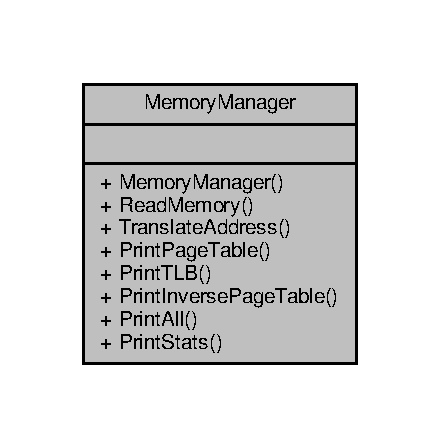
\includegraphics[width=211pt]{classMemoryManager__coll__graph}
\end{center}
\end{figure}
\subsection*{Public Member Functions}
\begin{DoxyCompactItemize}
\item 
\hyperlink{classMemoryManager_ae925e8ad4d8fe6f0565e9d5729f59593}{Memory\+Manager} ()
\begin{DoxyCompactList}\small\item\em Constructor. \end{DoxyCompactList}\item 
char \hyperlink{classMemoryManager_a4a716fc46ee321ebb25bd54bcc9d0524}{Read\+Memory} (int addr)
\begin{DoxyCompactList}\small\item\em Read a value from memory. \end{DoxyCompactList}\item 
int \hyperlink{classMemoryManager_a905ceff7ad39c05c2d965af613156547}{Translate\+Address} (int addr)
\begin{DoxyCompactList}\small\item\em Translate a virual address (P, d) to a physical address (f, d). Doesn\textquotesingle{}t implement any p. \end{DoxyCompactList}\item 
void \hyperlink{classMemoryManager_aa7437efdc1ebd09895d451e2c521857a}{Print\+Page\+Table} ()
\begin{DoxyCompactList}\small\item\em Print the page table. \end{DoxyCompactList}\item 
void \hyperlink{classMemoryManager_a4bc5f491976e5253bf00a07a71b55ef6}{Print\+T\+LB} ()
\begin{DoxyCompactList}\small\item\em Print the T\+LB. \end{DoxyCompactList}\item 
void \hyperlink{classMemoryManager_a231141529c907c50de129169f16bedf1}{Print\+Inverse\+Page\+Table} ()
\begin{DoxyCompactList}\small\item\em Print Inverse page table. \end{DoxyCompactList}\item 
void \hyperlink{classMemoryManager_ae7bbb5231788516ca34caca3d428b0ef}{Print\+All} ()
\begin{DoxyCompactList}\small\item\em Print T\+LB and Page Table. \end{DoxyCompactList}\item 
void \hyperlink{classMemoryManager_ad0c7c13901cb9c6844aebf6bf9238c47}{Print\+Stats} ()
\begin{DoxyCompactList}\small\item\em Print statistics for page faults and hit rate. \end{DoxyCompactList}\end{DoxyCompactItemize}


\subsection{Detailed Description}
A memory management unit. 

Definition at line \hyperlink{memory_8h_source_l00251}{251} of file \hyperlink{memory_8h_source}{memory.\+h}.



\subsection{Constructor \& Destructor Documentation}
\index{Memory\+Manager@{Memory\+Manager}!Memory\+Manager@{Memory\+Manager}}
\index{Memory\+Manager@{Memory\+Manager}!Memory\+Manager@{Memory\+Manager}}
\subsubsection[{\texorpdfstring{Memory\+Manager()}{MemoryManager()}}]{\setlength{\rightskip}{0pt plus 5cm}Memory\+Manager\+::\+Memory\+Manager (
\begin{DoxyParamCaption}
{}
\end{DoxyParamCaption}
)}\hypertarget{classMemoryManager_ae925e8ad4d8fe6f0565e9d5729f59593}{}\label{classMemoryManager_ae925e8ad4d8fe6f0565e9d5729f59593}


Constructor. 



Definition at line \hyperlink{memory_8cpp_source_l00291}{291} of file \hyperlink{memory_8cpp_source}{memory.\+cpp}.



\subsection{Member Function Documentation}
\index{Memory\+Manager@{Memory\+Manager}!Print\+All@{Print\+All}}
\index{Print\+All@{Print\+All}!Memory\+Manager@{Memory\+Manager}}
\subsubsection[{\texorpdfstring{Print\+All()}{PrintAll()}}]{\setlength{\rightskip}{0pt plus 5cm}void Memory\+Manager\+::\+Print\+All (
\begin{DoxyParamCaption}
{}
\end{DoxyParamCaption}
)}\hypertarget{classMemoryManager_ae7bbb5231788516ca34caca3d428b0ef}{}\label{classMemoryManager_ae7bbb5231788516ca34caca3d428b0ef}


Print T\+LB and Page Table. 



Definition at line \hyperlink{memory_8cpp_source_l00432}{432} of file \hyperlink{memory_8cpp_source}{memory.\+cpp}.

\index{Memory\+Manager@{Memory\+Manager}!Print\+Inverse\+Page\+Table@{Print\+Inverse\+Page\+Table}}
\index{Print\+Inverse\+Page\+Table@{Print\+Inverse\+Page\+Table}!Memory\+Manager@{Memory\+Manager}}
\subsubsection[{\texorpdfstring{Print\+Inverse\+Page\+Table()}{PrintInversePageTable()}}]{\setlength{\rightskip}{0pt plus 5cm}void Memory\+Manager\+::\+Print\+Inverse\+Page\+Table (
\begin{DoxyParamCaption}
{}
\end{DoxyParamCaption}
)}\hypertarget{classMemoryManager_a231141529c907c50de129169f16bedf1}{}\label{classMemoryManager_a231141529c907c50de129169f16bedf1}


Print Inverse page table. 



Definition at line \hyperlink{memory_8cpp_source_l00437}{437} of file \hyperlink{memory_8cpp_source}{memory.\+cpp}.

\index{Memory\+Manager@{Memory\+Manager}!Print\+Page\+Table@{Print\+Page\+Table}}
\index{Print\+Page\+Table@{Print\+Page\+Table}!Memory\+Manager@{Memory\+Manager}}
\subsubsection[{\texorpdfstring{Print\+Page\+Table()}{PrintPageTable()}}]{\setlength{\rightskip}{0pt plus 5cm}void Memory\+Manager\+::\+Print\+Page\+Table (
\begin{DoxyParamCaption}
{}
\end{DoxyParamCaption}
)}\hypertarget{classMemoryManager_aa7437efdc1ebd09895d451e2c521857a}{}\label{classMemoryManager_aa7437efdc1ebd09895d451e2c521857a}


Print the page table. 



Definition at line \hyperlink{memory_8cpp_source_l00424}{424} of file \hyperlink{memory_8cpp_source}{memory.\+cpp}.

\index{Memory\+Manager@{Memory\+Manager}!Print\+Stats@{Print\+Stats}}
\index{Print\+Stats@{Print\+Stats}!Memory\+Manager@{Memory\+Manager}}
\subsubsection[{\texorpdfstring{Print\+Stats()}{PrintStats()}}]{\setlength{\rightskip}{0pt plus 5cm}void Memory\+Manager\+::\+Print\+Stats (
\begin{DoxyParamCaption}
{}
\end{DoxyParamCaption}
)}\hypertarget{classMemoryManager_ad0c7c13901cb9c6844aebf6bf9238c47}{}\label{classMemoryManager_ad0c7c13901cb9c6844aebf6bf9238c47}


Print statistics for page faults and hit rate. 



Definition at line \hyperlink{memory_8cpp_source_l00441}{441} of file \hyperlink{memory_8cpp_source}{memory.\+cpp}.

\index{Memory\+Manager@{Memory\+Manager}!Print\+T\+LB@{Print\+T\+LB}}
\index{Print\+T\+LB@{Print\+T\+LB}!Memory\+Manager@{Memory\+Manager}}
\subsubsection[{\texorpdfstring{Print\+T\+L\+B()}{PrintTLB()}}]{\setlength{\rightskip}{0pt plus 5cm}void Memory\+Manager\+::\+Print\+T\+LB (
\begin{DoxyParamCaption}
{}
\end{DoxyParamCaption}
)}\hypertarget{classMemoryManager_a4bc5f491976e5253bf00a07a71b55ef6}{}\label{classMemoryManager_a4bc5f491976e5253bf00a07a71b55ef6}


Print the T\+LB. 



Definition at line \hyperlink{memory_8cpp_source_l00428}{428} of file \hyperlink{memory_8cpp_source}{memory.\+cpp}.

\index{Memory\+Manager@{Memory\+Manager}!Read\+Memory@{Read\+Memory}}
\index{Read\+Memory@{Read\+Memory}!Memory\+Manager@{Memory\+Manager}}
\subsubsection[{\texorpdfstring{Read\+Memory(int addr)}{ReadMemory(int addr)}}]{\setlength{\rightskip}{0pt plus 5cm}char Memory\+Manager\+::\+Read\+Memory (
\begin{DoxyParamCaption}
\item[{int}]{addr}
\end{DoxyParamCaption}
)}\hypertarget{classMemoryManager_a4a716fc46ee321ebb25bd54bcc9d0524}{}\label{classMemoryManager_a4a716fc46ee321ebb25bd54bcc9d0524}


Read a value from memory. 


\begin{DoxyParams}{Parameters}
{\em int} & Virtual address to read from. \\
\hline
\end{DoxyParams}

\begin{DoxyRetVals}{Return values}
{\em char} & value from mem\mbox{[}addr\mbox{]} \\
\hline
\end{DoxyRetVals}


Definition at line \hyperlink{memory_8cpp_source_l00299}{299} of file \hyperlink{memory_8cpp_source}{memory.\+cpp}.

\index{Memory\+Manager@{Memory\+Manager}!Translate\+Address@{Translate\+Address}}
\index{Translate\+Address@{Translate\+Address}!Memory\+Manager@{Memory\+Manager}}
\subsubsection[{\texorpdfstring{Translate\+Address(int addr)}{TranslateAddress(int addr)}}]{\setlength{\rightskip}{0pt plus 5cm}int Memory\+Manager\+::\+Translate\+Address (
\begin{DoxyParamCaption}
\item[{int}]{addr}
\end{DoxyParamCaption}
)}\hypertarget{classMemoryManager_a905ceff7ad39c05c2d965af613156547}{}\label{classMemoryManager_a905ceff7ad39c05c2d965af613156547}


Translate a virual address (P, d) to a physical address (f, d). Doesn\textquotesingle{}t implement any p. 


\begin{DoxyParams}{Parameters}
{\em int} & Virtual address to translate. \\
\hline
\end{DoxyParams}


Definition at line \hyperlink{memory_8cpp_source_l00403}{403} of file \hyperlink{memory_8cpp_source}{memory.\+cpp}.



The documentation for this class was generated from the following files\+:\begin{DoxyCompactItemize}
\item 
src/\hyperlink{memory_8h}{memory.\+h}\item 
src/\hyperlink{memory_8cpp}{memory.\+cpp}\end{DoxyCompactItemize}

\hypertarget{structMemoryPairAddress__t}{}\section{Memory\+Pair\+Address\+\_\+t Struct Reference}
\label{structMemoryPairAddress__t}\index{Memory\+Pair\+Address\+\_\+t@{Memory\+Pair\+Address\+\_\+t}}


{\ttfamily \#include $<$memory.\+h$>$}

\subsection*{Public Attributes}
\begin{DoxyCompactItemize}
\item 
int \hyperlink{structMemoryPairAddress__t_a5bc11426b27565b959f280dd1a18b080}{P}
\item 
int \hyperlink{structMemoryPairAddress__t_ad608e86288286889c2658e8043414edf}{d}
\end{DoxyCompactItemize}


\subsection{Detailed Description}


Definition at line \hyperlink{memory_8h_source_l00181}{181} of file \hyperlink{memory_8h_source}{memory.\+h}.



\subsection{Member Data Documentation}
\index{Memory\+Pair\+Address\+\_\+t@{Memory\+Pair\+Address\+\_\+t}!d@{d}}
\index{d@{d}!Memory\+Pair\+Address\+\_\+t@{Memory\+Pair\+Address\+\_\+t}}
\subsubsection[{\texorpdfstring{d}{d}}]{\setlength{\rightskip}{0pt plus 5cm}int Memory\+Pair\+Address\+\_\+t\+::d}\hypertarget{structMemoryPairAddress__t_ad608e86288286889c2658e8043414edf}{}\label{structMemoryPairAddress__t_ad608e86288286889c2658e8043414edf}


Definition at line \hyperlink{memory_8h_source_l00183}{183} of file \hyperlink{memory_8h_source}{memory.\+h}.

\index{Memory\+Pair\+Address\+\_\+t@{Memory\+Pair\+Address\+\_\+t}!P@{P}}
\index{P@{P}!Memory\+Pair\+Address\+\_\+t@{Memory\+Pair\+Address\+\_\+t}}
\subsubsection[{\texorpdfstring{P}{P}}]{\setlength{\rightskip}{0pt plus 5cm}int Memory\+Pair\+Address\+\_\+t\+::P}\hypertarget{structMemoryPairAddress__t_a5bc11426b27565b959f280dd1a18b080}{}\label{structMemoryPairAddress__t_a5bc11426b27565b959f280dd1a18b080}


Definition at line \hyperlink{memory_8h_source_l00182}{182} of file \hyperlink{memory_8h_source}{memory.\+h}.



The documentation for this struct was generated from the following file\+:\begin{DoxyCompactItemize}
\item 
src/\hyperlink{memory_8h}{memory.\+h}\end{DoxyCompactItemize}

\hypertarget{classPageTable}{}\section{Page\+Table Class Reference}
\label{classPageTable}\index{Page\+Table@{Page\+Table}}


Page table holding page/frame pairs.  




{\ttfamily \#include $<$memory.\+h$>$}

\subsection*{Public Member Functions}
\begin{DoxyCompactItemize}
\item 
\hyperlink{classPageTable_a75c92e794fd3f5397d2499d54dac22c9}{Page\+Table} ()\hypertarget{classPageTable_a75c92e794fd3f5397d2499d54dac22c9}{}\label{classPageTable_a75c92e794fd3f5397d2499d54dac22c9}

\begin{DoxyCompactList}\small\item\em Constructor for \hyperlink{classPageTable}{Page\+Table} object. \end{DoxyCompactList}\item 
int \hyperlink{classPageTable_a2590af90445c76b97420da95cf7210ec}{Lookup\+Page} (int pagenum)
\begin{DoxyCompactList}\small\item\em Lookup a page number and return the corresponding frame. \end{DoxyCompactList}\item 
void \hyperlink{classPageTable_ac961a37f5dde09c3addce2fcd118f24d}{Set\+Page\+To\+Frame} (int pagenum, int framenum)\hypertarget{classPageTable_ac961a37f5dde09c3addce2fcd118f24d}{}\label{classPageTable_ac961a37f5dde09c3addce2fcd118f24d}

\begin{DoxyCompactList}\small\item\em Set a page table entry to a given frame. \end{DoxyCompactList}\end{DoxyCompactItemize}


\subsection{Detailed Description}
Page table holding page/frame pairs. 

\subsection{Member Function Documentation}
\index{Page\+Table@{Page\+Table}!Lookup\+Page@{Lookup\+Page}}
\index{Lookup\+Page@{Lookup\+Page}!Page\+Table@{Page\+Table}}
\subsubsection[{\texorpdfstring{Lookup\+Page(int pagenum)}{LookupPage(int pagenum)}}]{\setlength{\rightskip}{0pt plus 5cm}int Page\+Table\+::\+Lookup\+Page (
\begin{DoxyParamCaption}
\item[{int}]{pagenum}
\end{DoxyParamCaption}
)}\hypertarget{classPageTable_a2590af90445c76b97420da95cf7210ec}{}\label{classPageTable_a2590af90445c76b97420da95cf7210ec}


Lookup a page number and return the corresponding frame. 


\begin{DoxyParams}{Parameters}
{\em page} & \\
\hline
\end{DoxyParams}

\begin{DoxyRetVals}{Return values}
{\em frame} & \\
\hline
\end{DoxyRetVals}


The documentation for this class was generated from the following files\+:\begin{DoxyCompactItemize}
\item 
src/memory.\+h\item 
src/memory.\+cpp\end{DoxyCompactItemize}

\hypertarget{classPhysicalMemory}{}\section{Physical\+Memory Class Reference}
\label{classPhysicalMemory}\index{Physical\+Memory@{Physical\+Memory}}


Imitates a physical memory.  




{\ttfamily \#include $<$memory.\+h$>$}

\subsection*{Public Member Functions}
\begin{DoxyCompactItemize}
\item 
\hyperlink{classPhysicalMemory_ad7fefaba61061c7339164836c6c02eaa}{Physical\+Memory} ()
\begin{DoxyCompactList}\small\item\em Constructor. Initializes memory to zero. \end{DoxyCompactList}\item 
int \hyperlink{classPhysicalMemory_a41ba2824ae9550b68036536d94ae8b32}{Find\+First\+Frame} ()
\begin{DoxyCompactList}\small\item\em Finds the first available frame in the memory. \end{DoxyCompactList}\item 
char \hyperlink{classPhysicalMemory_a2d6b5c45f2377838a76e58b2c083610a}{Get\+Memory\+Contents} (int frame, int offset)
\begin{DoxyCompactList}\small\item\em Gets the byte at position (f, d) \end{DoxyCompactList}\item 
bool \hyperlink{classPhysicalMemory_acde26e332e20349baa6c409b88635258}{is\+Full} ()
\begin{DoxyCompactList}\small\item\em Returns true/false if the memory is full/empty. \end{DoxyCompactList}\item 
void \hyperlink{classPhysicalMemory_a70cb4ae5b23f04cb347ac93cc9fc1028}{Page\+In} (int frame, char pagein\mbox{[}\hyperlink{memory_8h_af9b1b2ba12857a4bf11289dac8c5462d}{F\+R\+A\+M\+E\+\_\+\+S\+I\+ZE}\mbox{]})
\begin{DoxyCompactList}\small\item\em Pages a page into frame f. \end{DoxyCompactList}\item 
void \hyperlink{classPhysicalMemory_a6e1cf83f35ab25e879630783ebaecff3}{Page\+Out} (int frame)
\begin{DoxyCompactList}\small\item\em Page out a frame. \end{DoxyCompactList}\end{DoxyCompactItemize}


\subsection{Detailed Description}
Imitates a physical memory. 

Definition at line \hyperlink{memory_8h_source_l00041}{41} of file \hyperlink{memory_8h_source}{memory.\+h}.



\subsection{Constructor \& Destructor Documentation}
\index{Physical\+Memory@{Physical\+Memory}!Physical\+Memory@{Physical\+Memory}}
\index{Physical\+Memory@{Physical\+Memory}!Physical\+Memory@{Physical\+Memory}}
\subsubsection[{\texorpdfstring{Physical\+Memory()}{PhysicalMemory()}}]{\setlength{\rightskip}{0pt plus 5cm}Physical\+Memory\+::\+Physical\+Memory (
\begin{DoxyParamCaption}
{}
\end{DoxyParamCaption}
)}\hypertarget{classPhysicalMemory_ad7fefaba61061c7339164836c6c02eaa}{}\label{classPhysicalMemory_ad7fefaba61061c7339164836c6c02eaa}


Constructor. Initializes memory to zero. 



Definition at line \hyperlink{memory_8cpp_source_l00007}{7} of file \hyperlink{memory_8cpp_source}{memory.\+cpp}.



\subsection{Member Function Documentation}
\index{Physical\+Memory@{Physical\+Memory}!Find\+First\+Frame@{Find\+First\+Frame}}
\index{Find\+First\+Frame@{Find\+First\+Frame}!Physical\+Memory@{Physical\+Memory}}
\subsubsection[{\texorpdfstring{Find\+First\+Frame()}{FindFirstFrame()}}]{\setlength{\rightskip}{0pt plus 5cm}int Physical\+Memory\+::\+Find\+First\+Frame (
\begin{DoxyParamCaption}
{}
\end{DoxyParamCaption}
)}\hypertarget{classPhysicalMemory_a41ba2824ae9550b68036536d94ae8b32}{}\label{classPhysicalMemory_a41ba2824ae9550b68036536d94ae8b32}


Finds the first available frame in the memory. 


\begin{DoxyRetVals}{Return values}
{\em int} & Integer position of the first available frame. \\
\hline
\end{DoxyRetVals}


Definition at line \hyperlink{memory_8cpp_source_l00027}{27} of file \hyperlink{memory_8cpp_source}{memory.\+cpp}.

\index{Physical\+Memory@{Physical\+Memory}!Get\+Memory\+Contents@{Get\+Memory\+Contents}}
\index{Get\+Memory\+Contents@{Get\+Memory\+Contents}!Physical\+Memory@{Physical\+Memory}}
\subsubsection[{\texorpdfstring{Get\+Memory\+Contents(int frame, int offset)}{GetMemoryContents(int frame, int offset)}}]{\setlength{\rightskip}{0pt plus 5cm}char Physical\+Memory\+::\+Get\+Memory\+Contents (
\begin{DoxyParamCaption}
\item[{int}]{frame, }
\item[{int}]{offset}
\end{DoxyParamCaption}
)}\hypertarget{classPhysicalMemory_a2d6b5c45f2377838a76e58b2c083610a}{}\label{classPhysicalMemory_a2d6b5c45f2377838a76e58b2c083610a}


Gets the byte at position (f, d) 


\begin{DoxyParams}{Parameters}
{\em int} & Frame \# \\
\hline
{\em int} & Offset in bytes \\
\hline
\end{DoxyParams}

\begin{DoxyRetVals}{Return values}
{\em char} & Byte at (f, d) \\
\hline
\end{DoxyRetVals}


Definition at line \hyperlink{memory_8cpp_source_l00037}{37} of file \hyperlink{memory_8cpp_source}{memory.\+cpp}.

\index{Physical\+Memory@{Physical\+Memory}!is\+Full@{is\+Full}}
\index{is\+Full@{is\+Full}!Physical\+Memory@{Physical\+Memory}}
\subsubsection[{\texorpdfstring{is\+Full()}{isFull()}}]{\setlength{\rightskip}{0pt plus 5cm}bool Physical\+Memory\+::is\+Full (
\begin{DoxyParamCaption}
{}
\end{DoxyParamCaption}
)}\hypertarget{classPhysicalMemory_acde26e332e20349baa6c409b88635258}{}\label{classPhysicalMemory_acde26e332e20349baa6c409b88635258}


Returns true/false if the memory is full/empty. 


\begin{DoxyRetVals}{Return values}
{\em bool} & True if memory is full, False otherwise \\
\hline
\end{DoxyRetVals}


Definition at line \hyperlink{memory_8cpp_source_l00017}{17} of file \hyperlink{memory_8cpp_source}{memory.\+cpp}.

\index{Physical\+Memory@{Physical\+Memory}!Page\+In@{Page\+In}}
\index{Page\+In@{Page\+In}!Physical\+Memory@{Physical\+Memory}}
\subsubsection[{\texorpdfstring{Page\+In(int frame, char pagein[F\+R\+A\+M\+E\+\_\+\+S\+I\+ZE])}{PageIn(int frame, char pagein[FRAME_SIZE])}}]{\setlength{\rightskip}{0pt plus 5cm}void Physical\+Memory\+::\+Page\+In (
\begin{DoxyParamCaption}
\item[{int}]{frame, }
\item[{char}]{pagein\mbox{[}\+F\+R\+A\+M\+E\+\_\+\+S\+I\+Z\+E\mbox{]}}
\end{DoxyParamCaption}
)}\hypertarget{classPhysicalMemory_a70cb4ae5b23f04cb347ac93cc9fc1028}{}\label{classPhysicalMemory_a70cb4ae5b23f04cb347ac93cc9fc1028}


Pages a page into frame f. 


\begin{DoxyParams}{Parameters}
{\em int} & Frame \# to page into \\
\hline
{\em char\mbox{[}\+F\+R\+A\+M\+E\+\_\+\+S\+I\+Z\+E\mbox{]}} & Contents of the frame \\
\hline
\end{DoxyParams}


Definition at line \hyperlink{memory_8cpp_source_l00050}{50} of file \hyperlink{memory_8cpp_source}{memory.\+cpp}.

\index{Physical\+Memory@{Physical\+Memory}!Page\+Out@{Page\+Out}}
\index{Page\+Out@{Page\+Out}!Physical\+Memory@{Physical\+Memory}}
\subsubsection[{\texorpdfstring{Page\+Out(int frame)}{PageOut(int frame)}}]{\setlength{\rightskip}{0pt plus 5cm}void Physical\+Memory\+::\+Page\+Out (
\begin{DoxyParamCaption}
\item[{int}]{frame}
\end{DoxyParamCaption}
)}\hypertarget{classPhysicalMemory_a6e1cf83f35ab25e879630783ebaecff3}{}\label{classPhysicalMemory_a6e1cf83f35ab25e879630783ebaecff3}


Page out a frame. 


\begin{DoxyParams}{Parameters}
{\em int} & Frame to page out \\
\hline
\end{DoxyParams}


Definition at line \hyperlink{memory_8cpp_source_l00061}{61} of file \hyperlink{memory_8cpp_source}{memory.\+cpp}.



The documentation for this class was generated from the following files\+:\begin{DoxyCompactItemize}
\item 
src/\hyperlink{memory_8h}{memory.\+h}\item 
src/\hyperlink{memory_8cpp}{memory.\+cpp}\end{DoxyCompactItemize}

%--- End generated contents ---

% Index
\backmatter
\newpage
\phantomsection
\clearemptydoublepage
\addcontentsline{toc}{chapter}{Index}
\printindex

\end{document}
